%  Sujet 3 : Observations optiques et au MEB
% ==================================================================
\section[Observations optiques et au MEB]{Observations optiques et au MEB}

\subsection{Objectif}
L'objectif de ce sujet est de quantifier les profils d'\emph{undercut} des échantillons fabriqués au Sujet~2 (résine négative monocouche AZ nLOF 2070 vs système bicouche LOR 15C / ECI 3027) et de vérifier les dimensions critiques (CD) des pistes d'aluminium réalisées par \emph{lift-off} (Sujet~2) et par gravure (Sujet~4). On combine la microscopie optique pour les mesures latérales en vue de dessus et le MEB pour l'observation en coupe transversale \cite{prot3}.

\subsection{Matériels}
Le tableau~\ref{tab:s3-materiel} récapitule les échantillons et équipements utilisés lors de la séance.

\begin{table}[H]
  \centering\small
  \caption{Liste des échantillons et équipements utilisés pour le Sujet~3.}
  \label{tab:s3-materiel}
  \begin{tabularx}{\linewidth}{@{}l p{4.6cm} X@{}}
    \toprule
    \textbf{Catégorie} & \textbf{Matériel / Référence} & \textbf{Rôle dans le procédé} \\
    \midrule
    \textbf{Échantillons résines} & Wafers Si clivés du Sujet~2 (S1--S4) & Monocouche AZ nLOF 2070 (insolation S1 : \qty{58}{\second} ; S3 : \qty{62}{\second} avant/après +\qty{15}{\second} de sur-dév.) et bicouche LOR 15C / ECI 3027 (S2 : \qty{3}{\minute} ; S4 : \qty{5}{\minute}). \\
    \addlinespace[2pt]
    \textbf{Échantillons métal} & Wafer verre (Sujet~2) \& Wafer Si (Sujet~4) & Structures TLM en Ti/Al (\qty{10}{\nano\metre}/\qty{400}{\nano\metre}) issues du \emph{lift-off} (Sujet~2) et en Al issues de la gravure (Sujet~4). \\
    \addlinespace[2pt]
    \textbf{Microscopie optique} & Microscope optique \& logiciel de mesure & Contrôle visuel, mesure des rayons/largeurs (plans focaux $p$/$p'$) pour l'\emph{undercut} et mesure des pistes $W_{\text{opt}}$. \\
    \addlinespace[2pt]
    \textbf{Préparation MEB} & Pointe diamant \& Porte-échantillon incliné & Clivage des échantillons sélectionnés et montage incliné sur stub aluminium. \\
    \addlinespace[2pt]
    \textbf{Microscopie MEB} & MEB Hitachi TM-1000 (électrons rétrodiffusés, \qty{15}{\kilo\volt}) & Imagerie en coupe transversale et mesure des hauteurs de couches. \\
    \bottomrule
  \end{tabularx}
\end{table}

\subsection{Méthodes}

\paragraph{Étapes de caractérisation.}
La caractérisation s'effectue en trois étapes, illustrées par la figure~\ref{fig:s3-schema} :
\begin{enumerate}
  \item \textbf{Mesure optique de l'undercut :} Tous les échantillons (S1 à S4) sont inspectés au microscope optique. Pour l'AZ nLOF 2070 (S1, S3), on mesure la cote au sommet (plan focal $p$ : largeur $\text{top}$ ou rayon $R_{\text{ext}}$) et à la base (plan focal $p'$ : largeur $\text{bottom}$ ou rayon $R_{\text{int}}$) pour calculer le retrait latéral $u = (\text{top} - \text{bottom})/2 = R_{\text{ext}} - R_{\text{int}}$ et l'angle de pente $\alpha = \arctan(u / h)$, où $h$ est l'épaisseur Filmetrics du Sujet~2. Pour le système bicouche (S2, S4), le retrait $u$ sous l'ECI 3027 est mesuré en vue de dessus, soit directement comme largeur de la bande sombre (étoile, lignes), soit par différence des rayons (cercle de S4).
  \item \textbf{Coupe transversale au MEB :} Les échantillons présentant un \emph{undercut} sont clivés et montés sur un porte-échantillon incliné afin d'observer la tranche au MEB (Hitachi TM-1000, électrons rétrodiffusés) afin de mesurer les épaisseurs des couches et d'observer le surplomb.
  \item \textbf{Mesure optique des largeurs CD (motifs TLM) :} Sous les structures TLM, les largeurs réelles $W_{\text{opt}}$ des pistes d'aluminium ($W_{\text{mask}} =$ \qtyrange{10}{80}{\micro\metre}) sont mesurées au microscope optique sur l'échantillon \emph{lift-off} (Sujet~2) et sur l'échantillon gravé (Sujet~4).
\end{enumerate}

\begin{figure}[H]
  \centering
  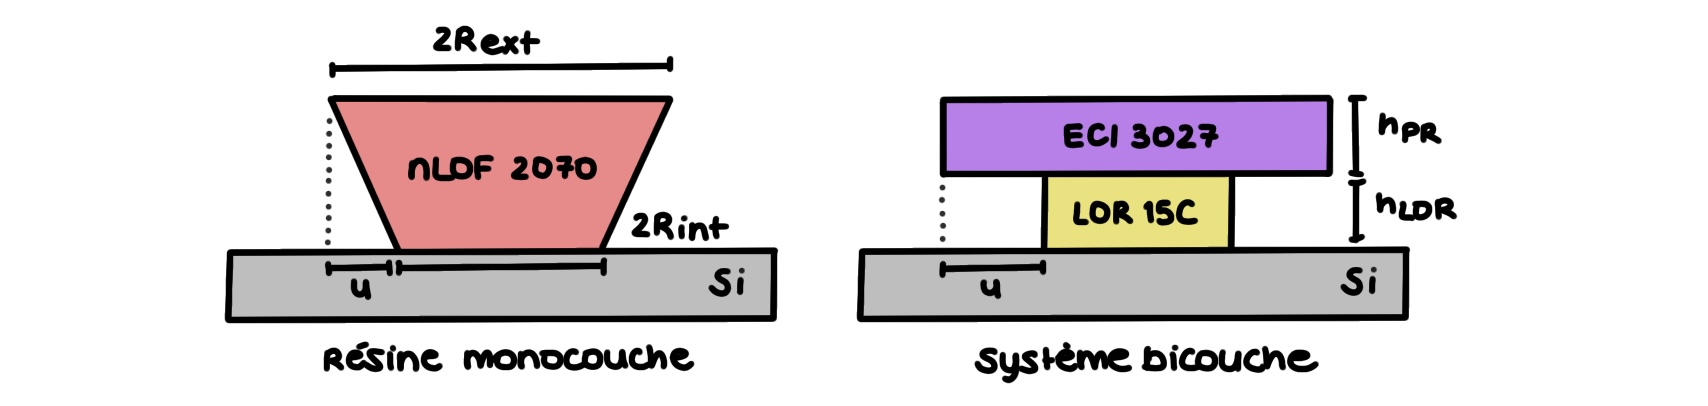
\includegraphics[width=\linewidth]{rapport-micro332/photos/s3_figure_prrocessus.jpg}
  \caption{Principe des mesures géométriques : à gauche, résine négative monocouche (diamètre $2R_{\text{ext}}$ au sommet, plan focal $p$, et $2R_{\text{int}}$ à la base, plan focal $p'$) ; à droite, coupe du système bicouche en surplomb.}
  \label{fig:s3-schema}
\end{figure}

\paragraph{Méthode de mesure.}
Les dimensions sont relevées directement avec les outils de mesure des logiciels d'acquisition (lignes parallèles, cercles ajustés ou mesure point-à-point au microscope ; cotes verticales au MEB).

\subsection{Résultats}

\paragraph{Mesures optiques des profils d'undercut.}
Les clichés métrologiques des échantillons S1 à S4 sont regroupés sur la figure~\ref{fig:s3-optique} et leurs dimensions sont synthétisées dans le tableau~\ref{tab:s3-optique}.

\begin{figure}[H]
  \centering
  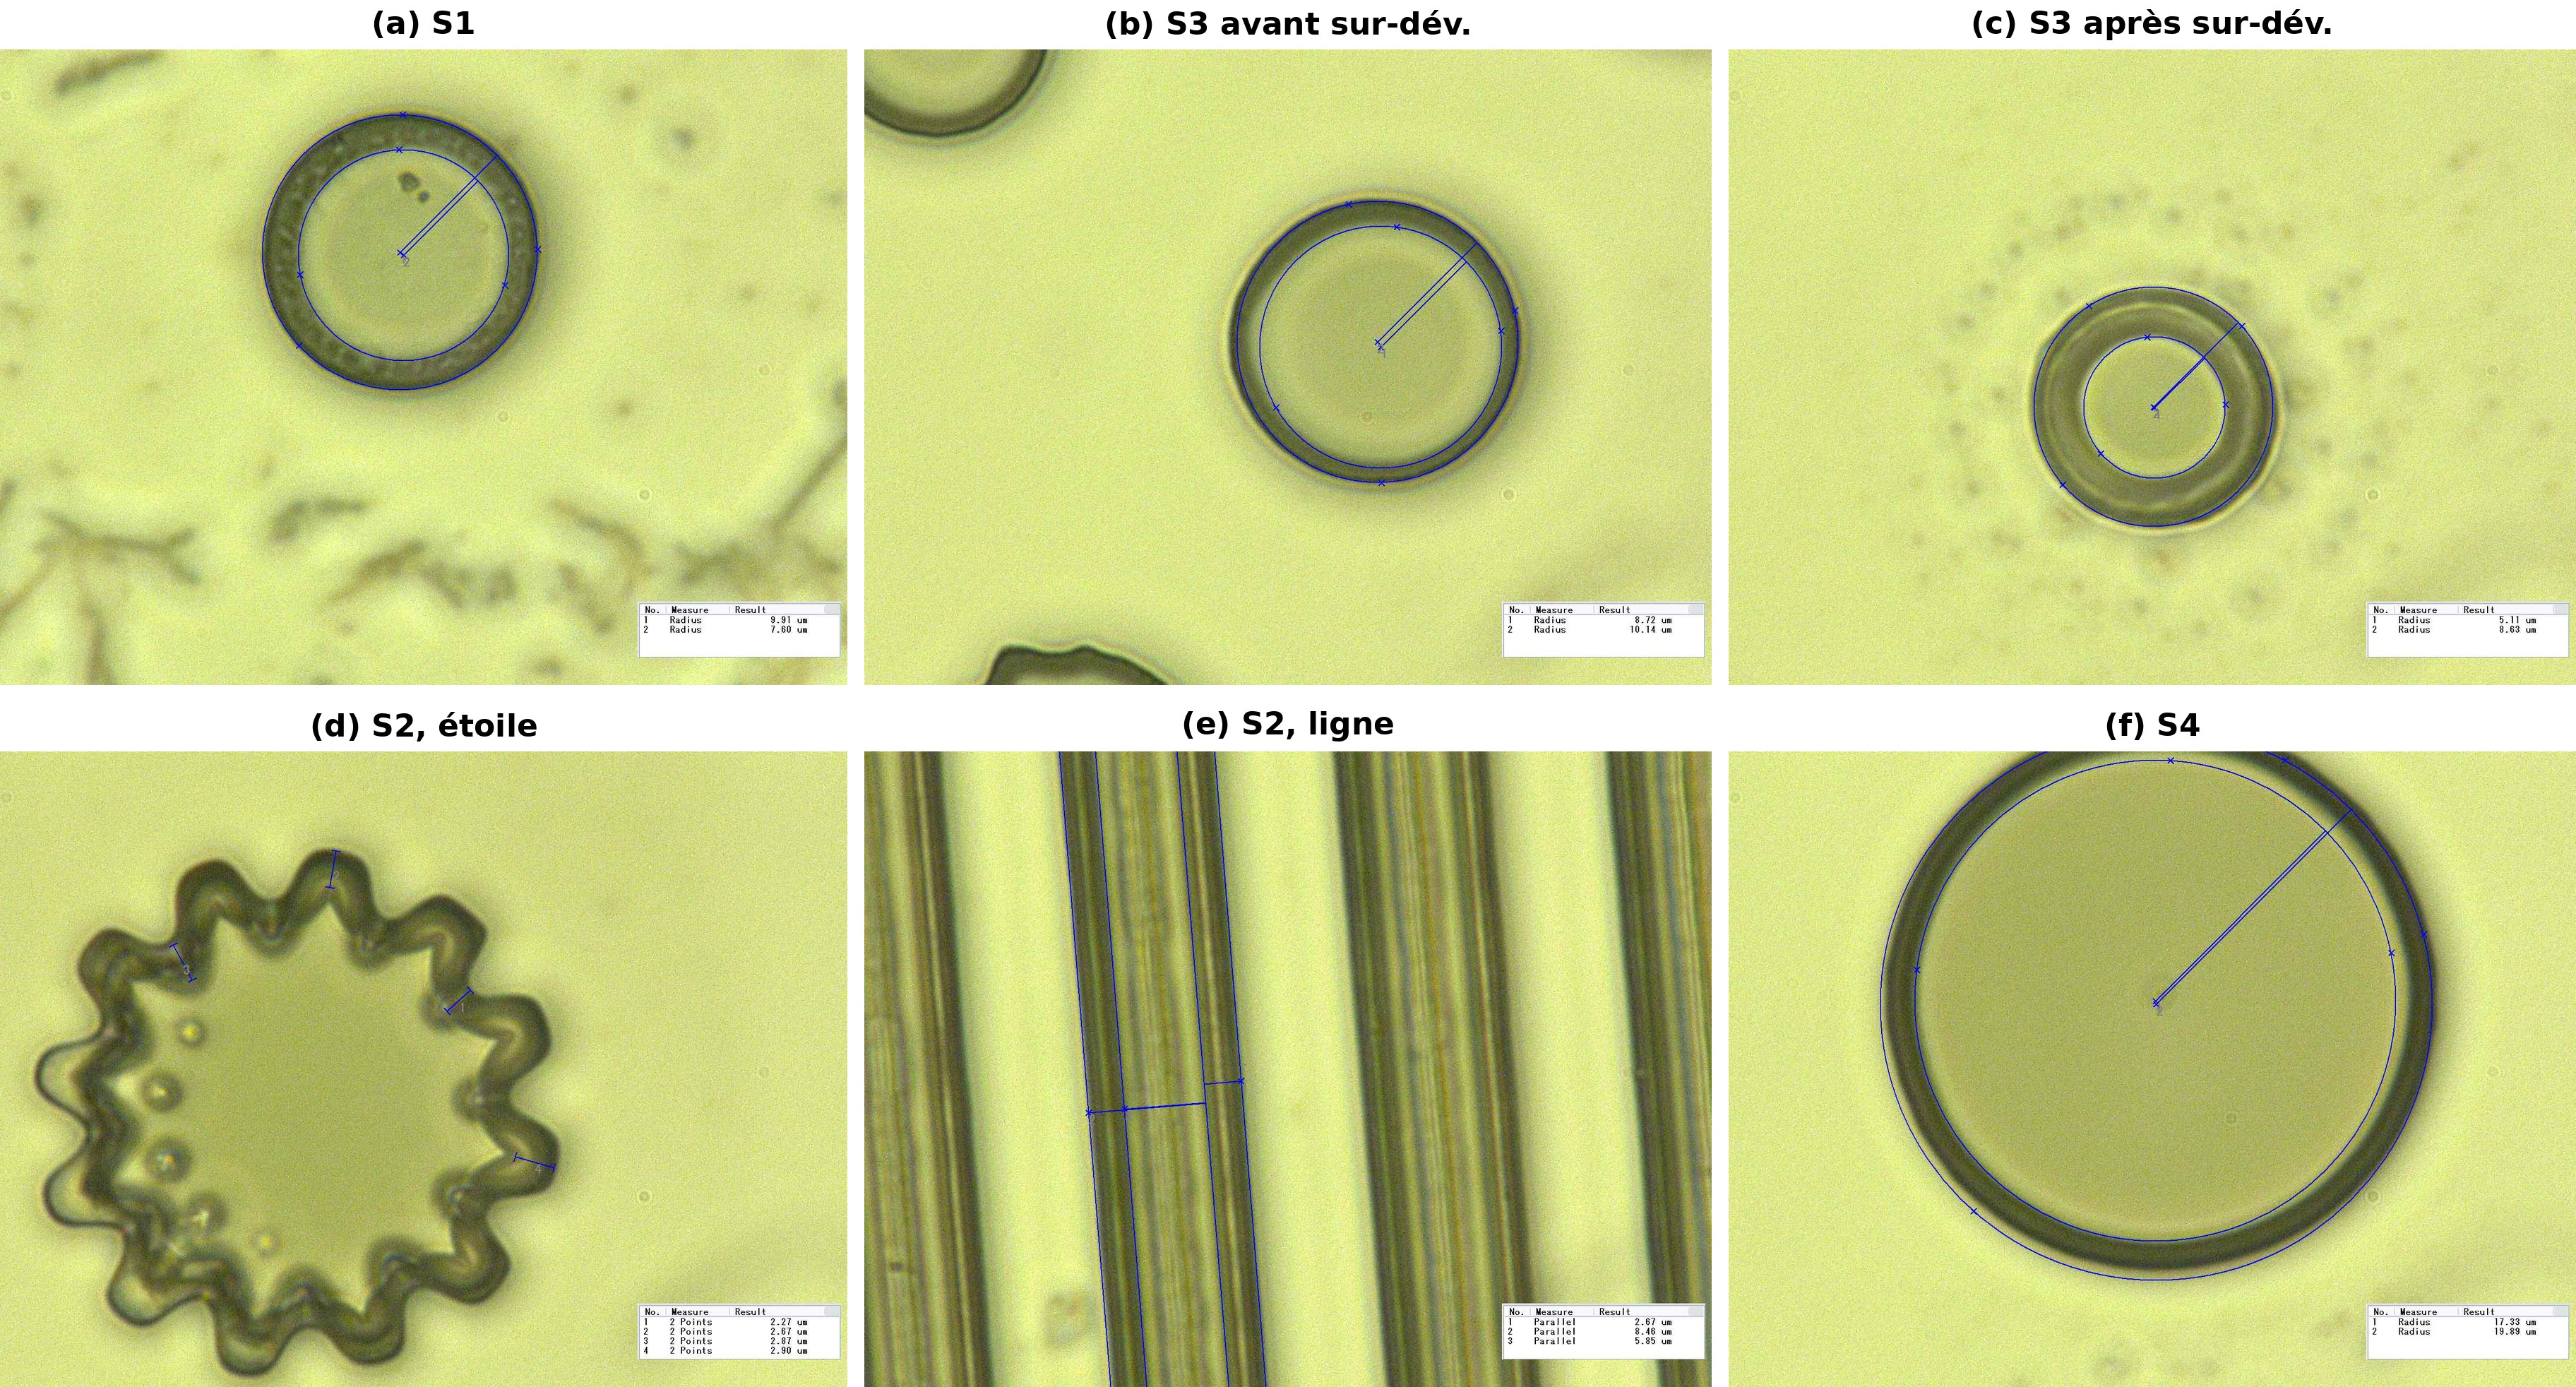
\includegraphics[width=\linewidth]{photos/fig3_2_optique_brut.jpg}
  \caption{Captures brutes au microscope optique avec les mesures du logiciel (encadré en bas à droite) : (a) S1 (nLOF, \qty{58}{\second}) ; (b) S3 avant sur-développement (\qty{62}{\second}) ; (c) S3 après +\qty{15}{\second} de sur-développement ; (d--e) S2 (bicouche, \emph{prebake} \qty{3}{\minute}) ; (f) S4 (bicouche, \emph{prebake} \qty{5}{\minute}).}
  \label{fig:s3-optique}
\end{figure}

\begin{table}[H]
  \centering\footnotesize
  \setlength{\tabcolsep}{3.5pt}
  \caption{Synthèse des mesures optiques de l'\emph{undercut} latéral $u$ et calcul de l'angle de pente $\alpha = \arctan(u/h)$.}
  \label{tab:s3-optique}
  \begin{tabularx}{\linewidth}{@{}X c c c c c c@{}}
    \toprule
    \textbf{Échantillon \& Motif} & \textbf{top} (\unit{\micro\metre}) & \textbf{bottom} (\unit{\micro\metre}) & $\mathbf{\Delta}$ (\unit{\micro\metre}) & $\mathbf{u}$ (\unit{\micro\metre}) & $\mathbf{h}$ (\unit{\micro\metre}) & $\mathbf{\alpha}$ (\unit{\degree}) \\
    \midrule
    \textbf{S1} (nLOF, \qty{58}{\second}) --- Cercle & 19,82 & 15,20 & 4,62 & \textbf{2,31}\textsuperscript{a} & 6,75 & \textbf{18,9} \\
    \textbf{S3} avant sur-dév. (\qty{62}{\second}) --- Cercle & 20,28 & 17,44 & 2,84 & \textbf{1,42} & 6,05 & \textbf{13,2} \\
    \textbf{S3} après +\qty{15}{\second} --- Cercle / Ligne & 17,26 & 10,22 & 7,04 & \textbf{3,52}\textsuperscript{b} & 6,05 & \textbf{30,2} \\
    \textbf{S2} (Bicouche, \qty{3}{\minute}) --- Étoile / Ligne & --- & --- & --- & \textbf{2,68}\textsuperscript{c} & 3,07 & --- \\
    \textbf{S4} (Bicouche, \qty{5}{\minute}) --- Cercle / Ligne & 39,78 & 34,66 & 5,12 & \textbf{2,56}\textsuperscript{d} & 2,91 & --- \\
    \bottomrule
  \end{tabularx}
  \vspace{2pt}
  \raggedright\scriptsize
  \textsuperscript{a}\,Mesure parallèle sur rectangle : \qty{1,76}{\micro\metre}.
  \textsuperscript{b}\,Mesure sur ligne : \qty{3,04}{\micro\metre}.
  \textsuperscript{c}\,Moyenne de 4 mesures directes sur l'étoile (\qtyrange{2,27}{2,90}{\micro\metre}) ; sur ligne, les deux bandes mesurent \qty{2,67}{\micro\metre} et \qty{2,61}{\micro\metre} (8,46 $-$ 5,85).
  \textsuperscript{d}\,Mesure sur ligne : \qty{2,38}{\micro\metre}. Pour S2 et S4, $h$ correspond à l'épaisseur du LOR 15C ; le profil est une marche (ECI en surplomb au-dessus du LOR) et non un flanc incliné, $\alpha$ n'est donc pas défini.
\end{table}

\paragraph{Observations en coupe transversale au MEB.}
Les clichés MEB acquis en vue inclinée (figure~\ref{fig:s3-meb}) illustrent la différence entre le flanc rétrograde continu de la résine négative AZ nLOF 2070 et le surplomb franc du système bicouche ECI 3027 / LOR 15C. Les cotes verticales mesurées sont résumées dans le tableau~\ref{tab:s3-meb}.

\begin{figure}[H]
  \centering
  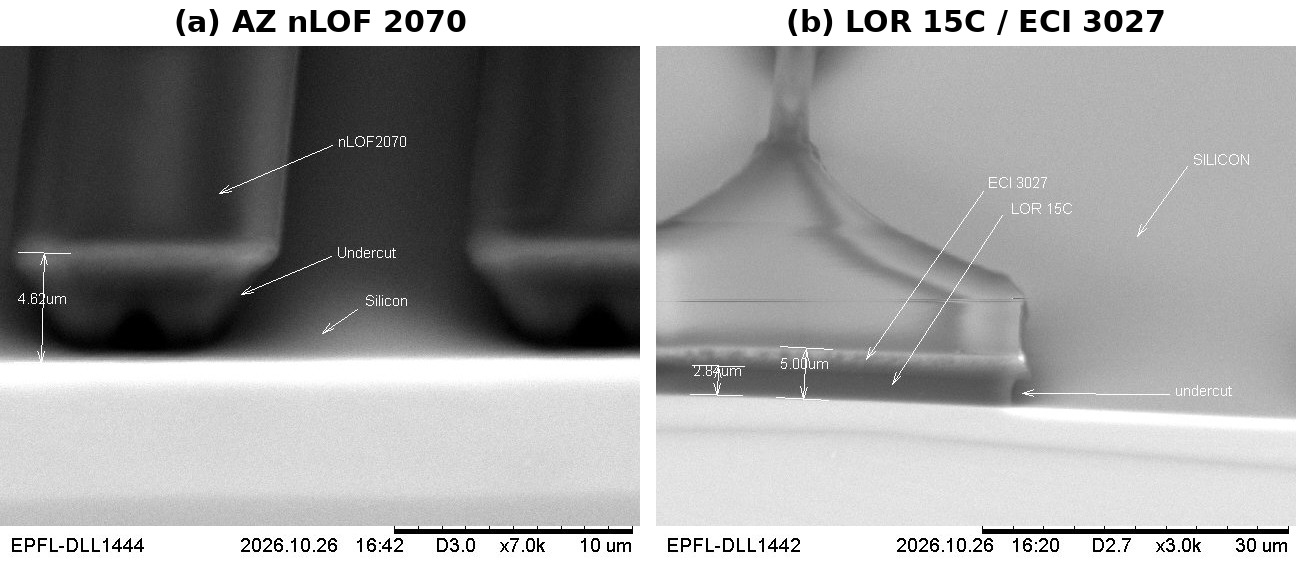
\includegraphics[width=\linewidth]{photos/fig3_3_meb_brut.jpg}
  \caption{Clichés MEB bruts (électrons rétrodiffusés, \qty{15}{\kilo\volt}, vue inclinée), avec les annotations et cotes faites pendant la séance : (a) flanc rétrograde continu de l'AZ nLOF 2070 ($\times 7{,}0\text{k}$, $h_{\text{app}} = \qty{4,62}{\micro\metre}$) ; (b) surplomb franc du bicouche ECI 3027 / LOR 15C ($\times 3{,}0\text{k}$, $h_{\text{LOR}} = \qty{2,84}{\micro\metre}$, $h_{\text{tot}} = \qty{5,00}{\micro\metre}$).}
  \label{fig:s3-meb}
\end{figure}

\begin{table}[H]
  \centering\footnotesize
  \caption{Dimensions verticales mesurées sur les clichés MEB en coupe et comparaison avec le Sujet~2.}
  \label{tab:s3-meb}
  \begin{tabularx}{\linewidth}{@{}X c c c@{}}
    \toprule
    \textbf{Grandeur mesurée en coupe MEB} & \textbf{Unité} & \textbf{Monocouche AZ nLOF 2070} & \textbf{Bicouche LOR 15C / ECI 3027} \\
    \midrule
    Hauteur couche inférieure ($h_{\text{LOR}}$) & \unit{\micro\metre} & --- & \textbf{2,84} \emph{(vs 2,91--3,07 Filmetrics)} \\
    Hauteur résine supérieure ($h_{\text{PR}}$) & \unit{\micro\metre} & \textbf{4,62} \emph{(projetée sous inclinaison)} & \textbf{2,16} \emph{(5,00 $-$ 2,84)} \\
    Hauteur totale ($h_{\text{tot}}$) & \unit{\micro\metre} & \textbf{4,62} \emph{(réelle 6,05--6,75)} & \textbf{5,00} \emph{(LOR + ECI)} \\
    Géométrie de l'\emph{undercut} & --- & Flanc incliné rétrograde continu & Surplomb horizontal franc (\emph{overhang}) \\
    \bottomrule
  \end{tabularx}
\end{table}

\paragraph{Mesure optique des largeurs de pistes TLM.}
Les largeurs optiques $W_{\text{opt}}$ des pistes d'aluminium mesurées sous les structures TLM (échantillon \emph{lift-off} du Sujet~2 et échantillon gravé du Sujet~4) sont rassemblées dans le tableau~\ref{tab:s3-tlm}. Aucune capture photographique n'a été enregistrée au microscope pour ces motifs lors de la séance.

\begin{table}[H]
  \centering\footnotesize
  \setlength{\tabcolsep}{4pt}
  \caption{Comparaison des largeurs optiques $W_{\text{opt}}$ des pistes d'aluminium TLM par rapport aux cotes nominales du masque $W_{\text{mask}}$ (Données empruntées au Groupe n°6 car nous n'avions pas les photos des pistes).}
  \label{tab:s3-tlm}
  \begin{tabularx}{\linewidth}{@{}X c c c c c c@{}}
    \toprule
    \textbf{Largeur nominale masque $W_{\text{mask}}$ (\unit{\micro\metre})} & \textbf{80} & \textbf{60} & \textbf{40} & \textbf{30} & \textbf{20} & \textbf{10} \\
    \midrule
    \textbf{Lift-Off (Sujet~2)} : $W_{\text{opt}}$ (\unit{\micro\metre}) & 82,6 & 62,8 & 42,1 & 32,0 & 21,4 & 10,9 \\
    \quad Écart $\Delta W = W_{\text{opt}} - W_{\text{mask}}$ (\unit{\micro\metre}) & $+2{,}6$ & $+2{,}8$ & $+2{,}1$ & $+2{,}0$ & $+1{,}4$ & $+0{,}9$ \\
    \quad Erreur relative (\%) & $+3{,}3$\,\% & $+4{,}7$\,\% & $+5{,}3$\,\% & $+6{,}7$\,\% & $+7{,}0$\,\% & $+9{,}0$\,\% \\
    \addlinespace[3pt]
    \textbf{Gravure (Sujet~4)} : $W_{\text{opt}}$ (\unit{\micro\metre}) & 80,0 & 59,5 & 36,4 & 26,8 & 16,9 & 7,4 \\
    \quad Écart $\Delta W = W_{\text{opt}} - W_{\text{mask}}$ (\unit{\micro\metre}) & $0{,}0$ & $-0{,}5$ & $-3{,}6$ & $-3{,}2$ & $-3{,}1$ & $-2{,}6$ \\
    \quad Erreur relative (\%) & $0{,}0$\,\% & $-0{,}8$\,\% & $-9{,}0$\,\% & $-10{,}7$\,\% & $-15{,}5$\,\% & $-26{,}0$\,\% \\
    \bottomrule
  \end{tabularx}
\end{table}

\FloatBarrier
\subsection{Analyse}

\paragraph{Analyse des données et des observations.}
\begin{enumerate}
  \item \textbf{Profils d'undercut en optique (tableau~\ref{tab:s3-optique}) :} Sur S1 (nLOF 2070, \qty{58}{\second}, $h = \qty{6,75}{\micro\metre}$), on mesure $u = \qty{2,31}{\micro\metre}$ sur cercle ($\alpha = \qty{18,9}{\degree}$) et \qty{1,76}{\micro\metre} sur rectangle. Sur S3 (\qty{62}{\second}, $h = \qty{6,05}{\micro\metre}$), la dose plus élevée limite le retrait initial à $u = \qty{1,42}{\micro\metre}$ ($\alpha = \qty{13,2}{\degree}$), mais le sur-développement de \qty{15}{\second} creuse la base jusqu'à $u = \qty{3,52}{\micro\metre}$ ($\alpha = \qty{30,2}{\degree}$). Pour le bicouche, S2 (\emph{prebake} \qty{3}{\minute}) atteint $u = \qty{2,68}{\micro\metre}$ en moyenne contre $u = \qty{2,56}{\micro\metre}$ pour S4 (\emph{prebake} \qty{5}{\minute}), avec la même insolation et le même développement. L'écart va dans le sens attendu, un LOR 15C moins recuit se gravant plus vite latéralement \cite{lor}, mais il reste du même ordre que la dispersion sur l'étoile (\qtyrange{2,27}{2,90}{\micro\metre}) et ne repose que sur deux échantillons.
  \item \textbf{Confrontation MEB et Filmetrics (tableau~\ref{tab:s3-meb}) :} Sur le système bicouche, la coupe MEB distingue nettement le LOR 15C ($h_{\text{LOR}} = \qty{2,84}{\micro\metre}$, en accord avec les \qtyrange{2,91}{3,07}{\micro\metre} Filmetrics) et l'ECI 3027 ($h_{\text{PR}} = \qty{2,16}{\micro\metre}$, total \qty{5,00}{\micro\metre}), avec une cavité d'\emph{undercut} franche à la base. Sur l'AZ nLOF 2070, le flanc est incliné de façon continue et la hauteur apparente (\qty{4,62}{\micro\metre}) est inférieure à l'épaisseur réelle (\qtyrange{6,05}{6,75}{\micro\metre}) du fait de l'inclinaison du porte-échantillon ($h_{\text{app}} = h_{\text{réel}}\sin\theta$, soit $\theta \approx$ \qtyrange{43}{50}{\degree} ; cet angle n'est pas enregistré par le MEB et nous le déduisons ici des épaisseurs Filmetrics). Les hauteurs du bicouche ne sont pas corrigées : leur accord avec le Filmetrics suppose que sa tranche a été vue presque de face.
  \item \textbf{Fidélité dimensionnelle des pistes TLM (tableau~\ref{tab:s3-tlm}) :} Les pistes obtenues par \emph{lift-off} sont systématiquement légèrement plus larges que le masque ($\Delta W$ compris entre $+0{,}9$ et \qty{+2,8}{\micro\metre}), tout en restant proches de la cote nominale même à \qty{10}{\micro\metre} (\qty{10,9}{\micro\metre}, soit $+9{,}0$\,\%). À l'inverse, la gravure humide réduit la largeur des pistes de \qtyrange{2,6}{3,6}{\micro\metre} pour $W_{\text{mask}} \le \qty{40}{\micro\metre}$ (soit environ \qtyrange{1,3}{1,8}{\micro\metre} de sous-gravure par côté), portant la perte relative à $-26{,}0$\,\% sur la piste de \qty{10}{\micro\metre} (\qty{7,4}{\micro\metre}). Les pistes très larges (\qty{80}{\micro\metre} et \qty{60}{\micro\metre}) présentent un écart quasi nul ($0{,}0$ à \qty{-0,5}{\micro\metre}). Une gravure isotrope devrait pourtant enlever la même largeur sur chaque bord, quelle que soit la piste : cet écart nul relève plutôt de la mesure (données du groupe~6, sans image pour la vérifier). Au sujet~6, le TLM du groupe~10 donne d'ailleurs une perte constante de \qty{2,5}{\micro\metre}, y compris à \qty{80}{\micro\metre}.
\end{enumerate}

\paragraph{Interprétation physique et discussion.}
Dans l'AZ nLOF 2070, la pente rétrograde ($\alpha = \qty{18,9}{\degree}$ à \qty{30,2}{\degree}) crée l'ombrage nécessaire lors de l'évaporation directionnelle, mais le sur-développement réduit l'assise au sol (sur S3, le diamètre à la base passe de \qty{17,44}{\micro\metre} à \qty{10,22}{\micro\metre}), fragilisant les motifs fins. Le système bicouche maintient une base large en LOR 15C sous un surplomb franc d'environ \qty{2,6}{\micro\metre} en ECI 3027, ce qui doit permettre une rupture nette du métal (S2 et S4 n'ont pas été métallisés). Sur les pistes TLM, le léger élargissement observé en \emph{lift-off} pourrait venir d'une ouverture au sommet de la résine un peu plus large que le masque, puisque c'est le bord du surplomb qui fixe la largeur du métal en évaporation directionnelle ; le TLM du sujet~6 (groupe~10) trouve au contraire des lignes à moins de \qty{1}{\micro\metre} de la cote du masque. Le rétrécissement en gravure résulte du caractère isotrope de l'attaque chimique humide sous le masque \cite{intro}. Enfin, la mesure optique se fait à travers la résine, en changeant de plan focal entre le sommet et la base, et le placement des bords reste approximatif : sur l'étoile de S2, nos quatre mesures vont de 2,27 à \qty{2,90}{\micro\metre}. Le MEB montre directement le profil en coupe, au prix d'une préparation destructive (clivage) et d'un risque de charge électrostatique des polymères ; nous n'y avons toutefois mesuré que des hauteurs, pas la largeur du surplomb.

\subsection{Conclusion}
La microscopie optique et le MEB ont permis de quantifier les profils d'\emph{undercut} du Sujet~2. Le sur-développement de \qty{15}{\second} sur S3 (\qty{62}{\second}) a porté son retrait latéral de \qty{1,42}{\micro\metre} ($\alpha = \qty{13,2}{\degree}$) à \qty{3,52}{\micro\metre} ($\alpha = \qty{30,2}{\degree}$), tandis que le système bicouche produit un surplomb régulier de \qtyrange{2,56}{2,68}{\micro\metre}, légèrement plus large pour le \emph{prebake} le plus court (\qty{3}{\minute} contre \qty{5}{\minute}), et dont la présence est confirmée en coupe MEB ($h_{\text{LOR}} = \qty{2,84}{\micro\metre}$). Sur les pistes TLM, le \emph{lift-off} assure une meilleure fidélité sur les motifs fins ($+9{,}0$\,\% à \qty{10}{\micro\metre}) que la gravure humide, dont la sous-gravure isotrope induit jusqu'à $-26{,}0$\,\% de perte de largeur.
